\item \textbf{{[}PJC/PRELIM/9597/2016/P1/Q4{]} }

A college uses a binary tree structure to store its subjects offered
to students. 

The program will use a user-defined type \texttt{Node} for each node
defined as follows: 
\begin{center}
\begin{tabular}{|l|l|l|}
\hline 
\texttt{\hspace{0.01\columnwidth}}Identifier & \texttt{\hspace{0.01\columnwidth}}Data Type & \texttt{\hspace{0.05\columnwidth}}Description\tabularnewline
\hline 
\texttt{Subject} & \texttt{STRING} & The node's value for subject offered\tabularnewline
\hline 
\texttt{LeftPtr} & \texttt{INTEGER} & The left pointer for the node\tabularnewline
\hline 
\texttt{RightPtr} & \texttt{INTEGER} & The right pointer for the node\tabularnewline
\hline 
\end{tabular}
\par\end{center}

A linked list is maintained of all unused nodes which do not form
part of the tree. The first available node which is used for a new
item is indicated by NextFreePosition. Items in the unused list are
linked using their left pointers. 

The binary tree and linked list are implemented using variables as
follows: 
\begin{center}
\begin{tabular}{|l|l|l|}
\hline 
\texttt{\hspace{0.01\columnwidth}}Identifier & \texttt{\hspace{0.01\columnwidth}}Data Type & \texttt{\hspace{0.05\columnwidth}}Description\tabularnewline
\hline 
\texttt{SubjectTree} & \texttt{STRING} & The tree data\tabularnewline
\hline 
\texttt{Root} & \texttt{INTEGER} & Index position of the root node\tabularnewline
\hline 
\texttt{NextFreePosition} & \texttt{INTEGER} & Index for the next unused node\tabularnewline
\hline 
\end{tabular}
\par\end{center}

The diagram shows the binary tree and linked list after five subjects
have been added.
\begin{center}
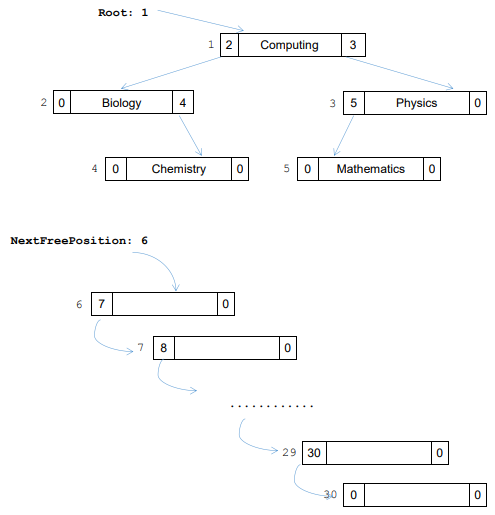
\includegraphics[width=0.5\paperwidth]{C:/Users/Admin/Desktop/Github/question_bank/LyX/static/img/9597-PJC-2016-P1-Q4-1}
\par\end{center}

\subsection*{Task 4.1 }

Write the program code to declare all the required variables and create
the initial linked list which contains all 30 nodes. 

Add statement(s) to initialise the empty tree. 

\subsection*{Evidence 16: }

Your program code for task 4.1. \hfill{}{[}8{]}

The following incomplete pseudocode inserts a data value into the
binary tree structure.

\noindent %
\noindent\begin{minipage}[t]{1\columnwidth}%
\texttt{PROCEDURE InsertBinaryTree(NewItem)}

\texttt{\qquad{}... ... }

\texttt{\qquad{}IF tree is empty }

\texttt{\qquad{}\qquad{}THEN }

\texttt{\qquad{}\qquad{}\qquad{}... ...}

\texttt{\qquad{}ELSE}

\texttt{\qquad{}\qquad{}//traverse the tree to find the insert position }

\texttt{\qquad{}\qquad{}... ... }

\texttt{\qquad{}\qquad{}LastMove = 'X'}

\texttt{\qquad{}\qquad{}REPEAT}

\texttt{\qquad{}\qquad{}\qquad{}PreviousPtr <- CurrentPtr }

\texttt{\qquad{}\qquad{}\qquad{}IF NewItem < CurrentPtr item}

\texttt{\qquad{}\qquad{}\qquad{}\qquad{}THEN }

\texttt{\qquad{}\qquad{}\qquad{}\qquad{}\qquad{}//move left}

\texttt{\qquad{}\qquad{}\qquad{}\qquad{}\qquad{}CurrentPtr <-
CurrentPtr's left pointer}

\texttt{\qquad{}\qquad{}\qquad{}\qquad{}\qquad{}LastMove = 'Left' }

\texttt{\qquad{}\qquad{}\qquad{}\qquad{}ELSE}

\texttt{\qquad{}\qquad{}\qquad{}\qquad{}\qquad{}//move right }

\texttt{\qquad{}\qquad{}\qquad{}\qquad{}\qquad{}CurrentPtr <-
CurrentPtr's right pointer }

\texttt{\qquad{}\qquad{}\qquad{}\qquad{}\qquad{}LastMove = 'Right'}

\texttt{\qquad{}\qquad{}\qquad{}ENDIF }

\texttt{\qquad{}\qquad{}UNTIL CurrentPtr = NULL }

\texttt{\qquad{}ENDIF }

\texttt{\qquad{}IF LastMove = 'Left'}

\texttt{\qquad{}... ... }

\texttt{\qquad{}ELSE IF LastMove = 'Right'}

\texttt{\qquad{}... ...}

\texttt{\qquad{}ENDIF }

\texttt{\qquad{}... ... }

\texttt{END PROCEDURE }%
\end{minipage}

\subsection*{Task 4.2 }

Complete the pseudocode and write a module \texttt{AddSubject} to
add a subject into the binary tree. 

\subsection*{Evidence 17:}

Your \texttt{AddSubject} program code. \hfill{} {[}7{]}

\subsection*{Task 4.3 }

Write a module \texttt{Display} to display the value of \texttt{Root},
the value of \texttt{NextFreePosition} and the contents of \texttt{SubjectTree}
in index order. 

\subsection*{Evidence 18: }

Your \texttt{Display} program code. \hfill{} {[}4{]}

\subsection*{Task 4.4}

Write a module \texttt{BuildTree} to construct a binary tree using
the data provided in the data file \texttt{SUBJECT.TXT}. Read in all
the data from the data file and use the \texttt{AddSubject} module. 

\subsection*{Evidence 19: }

Your \texttt{BuildTree} program code. \hfill{}{[}2{]}

\subsection*{Evidence 20:}

Run your program and produce screenshot of contents of binary tree.
\hfill{} {[}1{]}

Deleting a node from a tree may change the structure of the tree.
To simplify the deletion process, label a node as \textquotedblleft \texttt{deleted}\textquotedblright{}
but \textbf{do not remove the node} from the tree structure. After
that, regenerate the entire tree structure.

\subsection*{Task 4.5 }

Write a module \texttt{LabelDelete} that labels a node as \textquotedblleft \texttt{deleted}\textquotedblright{}
but do not remove the node from the tree structure. 

\subsection*{Evidence 21: }

Your LabelDelete program code. \hfill{}{[}6{]}

\subsection*{Task 4.6}

Write program code to regenerate the entire binary tree.

\subsection*{Evidence 22: }

Your program code to regenerate the binary tree. \hfill{}{[}6{]}

\subsection*{Evidence 23:}

Display a screenshot of the regenerated binary tree after deleting
\textquotedblleft \texttt{Chemistry}\textquotedblright{} and \textquotedblleft \texttt{History}\textquotedblright .
\hfill{} {[}1{]}